\chapter{自然语言处理的研究现状}{The State of the Art in Natural Language Processing}
\label{chap:review}

     近年来,自然语言处理(NLP)逐渐成为人们越来越关注的领域。它融合了计算机科学、语言学,以及其它学科。本文涉及了NLP领域中各个不同的研究方向,因此无法在短篇幅内给出每个方向的所有相关文献综述。Jurafsky的书 \cite{Jurafsky2009}已对这一领域进行了概述。在这一章中,我们将对众多NLP相关领域的研究现状进行大致的回顾,同时对NLP中的几个与我们的工作密切相关,或者具有可比性的研究方向和理论进行比较深入的探讨。在简要的研究历史回顾后,我们会总结自然语言理解、自然语言生成、对话系统、以及语义上的知识表示方面的未来发展趋势以及主要存在的问题。

\section{关于有效的可计算的语言处理的探索}{The Quest for Effective Computational Language Processing}

      从人工智能发展的早期开始,人们已认识到NLP在机器智能领域的关键性作用。在1950年,Alan Turing发表了他的那篇经典文章“计算机与智能化(Computing  Machinery and Intelligence)”。在文章中,他提出了一个理论,现在我们称其“作为智能标准的图灵测试”。他并没有称之为“自然语言处理”,但对于任何系统来说,要通过图灵测试,NLP显然是至关重要的。

人工智能方面的先驱在早期过于乐观,在自然语言处理方面也是如此。1954年,乔治城大学(Georgetown University)进行了一项试验,他们利用机器翻译将60多个俄语句子翻译成英文。这个试验的发起人声称:在3年或5年内,机器翻译将不成问题。然而,到1966年,一份报告显示:持续10年的研究都没有取得多少进展,而用于机器翻译的研究资金也大幅减少。事实上,在之后的15-20年里,机器翻译一直停滞不前,直到人们发现了完全不同的“统计语料库”分析法。
通过基于规则的对话系统,人们取得了初步进展。例如聊天机器人心理医生ELIZA\cite{Weizenbaum1966}和用于受限“积木世界(blocks worlds)” 的自然语言系统SHRDLU\cite{Winograd1972}。图 \ref{fig:eliza}中是ELIZA的对话例句。

\begin{figure}[htb]
\centering
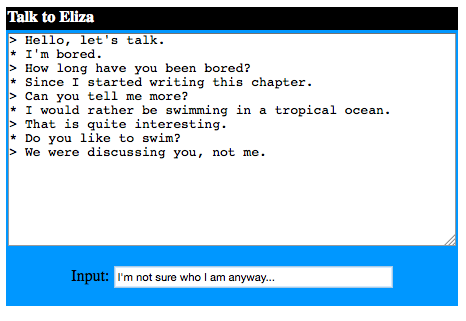
\includegraphics[width=14cm]{figures/eliza.png}
\caption{ 对话例句。这是与知名的聊天机器人心理医生ELIZA对话的现代版本。请注意:当“她”不知道该怎样回答的时候,“她”是如何转移话题的。 }
\label{fig:eliza}
\end{figure}

尽管这些系统看起来很聪明,甚至有些像人类的思维,但它们显然缺乏对它们所使用的语言的深度理解,而且至今,类似的对话系统也没有比这些早期的原型系统懂的更多。

在20世纪70年代,为了克服早期这些基于规则的聊天机器人的缺陷,许多程序员开始编写“概念本体知识库”,这些知识库将真实世界的信息转换为计算机可以理解的数据,以便聊天机器人获得更多的知识 \cite{McCorduck2004}。相对来说,在20世纪70年代早期,基于知识本体的“问答”(QA)系统在限定的领域内是成功的,例如LUNAR系统。它能够回答那些对阿波罗登月任务 \cite{Woods1973} 中带回的岩石进行地质分析的问题。(例如:高碱性岩石中铝元素的平均浓度是多少?)。 1971年的月球科学会议展示了LUNAR系统。当时,对于没有经过该领域训练的人提出的相关问题,LUNAR能够答出90\%。在之后的几年间,更多基于限定领域的问答系统相继出现。这些系统的共同特点是:都有核心数据库,或由相关领域的专家人工编写的知识系统。LUNAR和当时其它一些系统的语言能力只能与ELIZA的语言能力相提并论。

经过20世纪70年代和80年代的发展,NLP系统已能够融入了更先进的语言学理论,例如20世纪80年代末期,由加州伯克利大学Robert Wilensky 教授开发的Unix Consultant (UC)\cite{Wilensky88theberkeley}。UC以大量人工书写的知识库为基础,可以回答与Unix操作系统有关的问题。它会根据它对不同对话人所提出的问题的理解,组合出不同的答案。这种系统正是目前受限领域的自然语言问答系统(例如用于健康和生命科学的EAGLi \cite{eagli})的前身。

在这一时期,理论语言学和实用计算NLP之间的关系是错综复杂的,甚至有些麻烦。主流的理论语言学主要是基于Noam Chomsky的理论,这个理论的中心是:假定句子的“表层结构”能微妙地转换成“深层句法结构”。尽管人们进行了大量尝试,但发现这些理论并不适合计算机应用\cite{McCorduck2004}。

在NLP的发展历程中,最具革命性的事件是大型文本和语音语料库的出现,以及统计分析方法的发展。基于统计的NLP的目标是通过识别和判定这些语料库中的各种模式,来实现语言处理功能。这些方法的流行主要是由于计算机和通讯技术的进步,以及人们越来越多地使用光盘,紧接着互联网,而并不是因为NLP本身的发展。由于人们对作为训练语料库的平行文本语料库的使用,并在训练语料库上使用相对简单的统计学习算法,例如基于隐马尔科夫模型 (HMMs)\cite{Hutchins2005},机器翻译出现了重大进展。由Chomsky的早期导师Zellig Harris \cite{Harris1957}引领的标注语料库创建工作在众多实践中脱颖而出,同时一个有助于“有监督学习”任务的大规模分支领域出现了。例如:利用统计工具从标注语料库中学习语法,语料库中的每个句子都有人工标注的句法结构;或者使用人工标注的词性标注语料库,利用统计工具对新的文本进行自动词性标注。

“从大规模语料库中进行无监督学习”也是自然语言处理的研究重点(例如\cite{Spitkovsky2013}),但事实证明这更加困难。而“半监督式学习”则是相对成功的。它融合了标注语料库和网络中大量非标记文本的使用\cite{Abney2007} \cite{Guo2014}。


\section{自然语言理解}{Comprehension}

自然语言理解是NLP的分支领域,它是通过使用软件来理解自然语言的意义(语音,或者本文更关注的“文本”)。自然语言理解主要是将自然语言转换成抽象的语义形式,以获取语言的含义;或者是转换为某种响应(例如对某个问题的回答),以说明其理解了语言的含义。

\subsection{句法分析}{Syntactic Parsing}

通常自然语言理解是通过对句子的某些,或全部句法法进行分析来完成的。大量的形式化体系和算法通过它们自己的独特方式对句子的句法结构进行解析。大体来说,这些可以归类为“依存语法(DG)”对“短语结构语法(PSG)”。PSG首先对句子进行短语分析,然后指出单词和短语之间的关系,以及短语之间的关系;另一方面,DG仅仅在句子中的单词之间标注(有标记的)连接关系。后者(DG)是我们要在本文中探讨的语法类型。


这里的“依存”是指语言单位(如单词)由有向链接相互联系在一起。一般来说,在DG中,(限定)动词被视为句子或子句结构的中心,其它所有句法单位(单词)是直接或间接地与动词通过有向链接相连。这种有向链接被称为“依存”。句子结构是由一个词(中心词)与它的依存词之间的关系而决定的。


“依存”关系是一对一的对应关系:对于句子中的每个元素(例如:单词或语素)来说,实际上句子中都有一个与其相对应的节点。这种一对一的对应关系决定了“依存语法”就是单词(或语素)的语法。所有的句子都有元素和将元素组成结构的依存关系,这种情况应该与短语结构语法的“成分关系”进行比较,“成分关系”是一对一,或一对多的对应关系,也就是说,对于句子中的每个元素来说,有一个或多个与其对应的节点。这种不同带来的结果是:相比短语结构,依存结构非常紧凑,因为它往往包含很多小的节点。从计算机处理的角度来说,这种简洁的结构是有益的。


\subsection{关系抽取}{Relationship Extraction}
自然语言理解中的一个重要方向是{\bf 关系抽取}。在NLP领域中,关系抽取已成为一个重要的研究方向,一方面是因为它的实际应用价值,另一方面因为它被看做是语义分析的一部分,而且是目前的技术相对容易实现的那部分。到目前为止,吸引最多注意力的关系抽取是命名实体之间的关系识别,例如:“个人从属关系”和“组织地址关系”。

一般来说,关系可以由一个元组的形式来定义的,$t = (e_1, e_2, ...,e_n)$。在这里,$e_i$ 是文本中预定义关系$r$ 的实体。大多数关系抽取系统主要关注二元关系的抽取。例如 :

\begin{verbatim}
位于(厦门,中国)
father-of(Richard Li, Li Ka-Shing)
\end{verbatim}

抽取“高阶关系”也非常有意义。例如这个句子:``At codons 12, the occurence of point mutations from G to T were observed'' (“在密码子12,观察到从G到T的点突变”)。句子中出现了一个4进制生物医学关系,可以描述为:

\begin{verbatim}
point mutation(codon, 12, G, T)
\end{verbatim}

目前人们普遍视“关系抽取”为一个有监督分类问题,它从一个语料库开始(语料库中包含由人类标记的相关语义关系),然后利用统计方法来对标记的关系建模,并学习出适合应用于其它文本的统计模型。

目前,关系抽取系统的主要限制在句子层面上运用。事实上,关系可能跨越句子,甚至贯穿不同的文件。然而,解决这一问题需要一定的常识和非常灵活的知识表示。本文的研究也无法直接解决这一问题,但我们相信:通过将句子意义映射为通用的知识表示,我们已经奠定了解决问题的基础。在这种知识表示中,跨句或跨文本的通用联系和推理是可以被实现的。

\subsection{流结构语法}{Fluid Construction Grammar}

将流结构语法(FCG)与本文使用的语言形式化体系进行比较分析是很有意义的。在FCG中,一句话语的信息是以语义和句法结构组织在一起的。语义结构是对“话语意思”的分解,它含有特定语言的语义分类,例如:“put”事项被归类为“起因-移动-位置”类事项,包括一个施事者(agent)、一个受事者(patient)和一个位置(location)。句法结构是将话语形式分解为成分和词素,还包含附加的句法分类,比如:句法特征(例如:数量和性别)、词序限制等。


从理论上来说,FCG是基于一种程序性语义的方法,在这个意义上,话语的意思是听话人假定要执行的程序,因此,概念化便是一个规划过程(规划该程序),而解析便是对该程序的执行过程。
FCG中,有关配对句法和语义结构的例子(短语“the ball”),请见图 \ref{fig:fcg1} and \ref{fig:fcg2}。

\begin{figure}[htb]
\centering
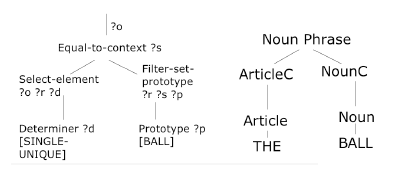
\includegraphics[width=12cm]{figures/fcg1.png}
\caption{ FCG syntactic and semantic structure for "the ball" }
\label{fig:fcg1}
\end{figure}

\begin{figure}[htb]
\centering
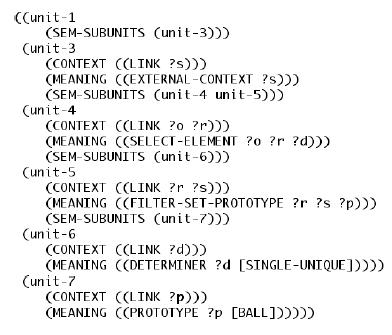
\includegraphics[width=12cm]{figures/fcg2.png}
\caption{ FCG semantic structure for "the ball" in  list format}
\label{fig:fcg2}
\end{figure}


所有的FCG规则都是双向的。通常在产生过程中,所要表达的语义内容是与语义结构相统一的,有可能产生一组绑定。如果成功了,绑定会与语义结构相融合。这种融合可以理解为“部分统一”,但它利用结构中那些遗漏部分扩展了结构。在句法分析过程中,被分析的句子与句法结构是统一的,同时,结果中的某些部分被添加到语义结构中。


这篇论文所提出的形式化体系在概念上有些类似FCG。 此外,我们有配对句法和语义结构,而且还进行双向处理。在第\ref{chap:comprehension}章中,我们将论述链语法,它将句子转换成句法结构,以及RelEx和RelEx2Logic模块,它们将句法结构转换成语义结构。在第 \ref{chap:generation}章中,我们将论述Microplanner 和SuReal模块,从另一个方向,将语义结构转换成句法结构,再生成句子。OpenCog中的模式匹配器(Pattern Matcher)使用我们的句法和语义结构时,也将这些结构视为有效的程序,同样实现了“程序性语义”。

我们的形式化体系与FCG的着重点不同。FCG主要是用作探索问题的理论工具,而我们所做的OpenCog系统则是用于真实世界的实际应用。

\section{知识表示}{Knowledge Representation}

对于任何以实现复杂功能(如对话系统或复杂的问答系统)为目标的NLP系统来说,该系统如何表达内部知识是非常关键的。先进的NLP功能一般要求从多个句子中获得互相关的信息,这通常需要持续存储那些从多个句子中抽取的信息。这种存储机制必须能够支持相当灵活的语义知识操作。上节我们看到的例子是FCG使用的基于逻辑的语义表达形式。在本文的研究中,我们将使用一种不同的逻辑表达形式,即OpenCog中概率逻辑网PLN(Probaabilistic Logic Networks)的形式体系。

\subsection{逻辑知识表示的优缺点}{Strengths and Weaknesses of Logical Knowledge Representation}

根据Pei Wang \cite{Wang2006}的理论,总体来说,逻辑推理系统通常包括以下组成部分:

\begin{itemize}
\item 一种形式化语言, 能用于知识表示,以及系统与其环境之间的沟通。
\item 一个语义系统,用于决定词的意义和句子真值。
\item 一套推理规则,匹配问题和知识,能从前提推出结论等。
\item 一个存储器,可以储存问题和知识,并提供推理的工作空间。
\item 一个控制机制,负责选择前提和每一步推理中需要的推理法则。
\end{itemize}

\noindent 前3个通常被认为是逻辑,或推理系统中的逻辑部分,最后的2个则被认为是推理系统中的控制部分。

使用逻辑来表达自然语言的语义,这涉及精确度和灵活度之间的平衡。逻辑是精确的,它的标志是“确定”。它带来一种用作定理证明的思考方式。它的优势在于稳定和系统的方式对表达式赋值并保持表达式的真值。在几乎没有歧义的技术领域,精确度是非常重要的,而逻辑显然是一个极好的架构。但是,当逻辑在意思和真值都比较模糊和模棱两可的领域中应用时,其适用性就不那么明显了,而且在人工智能和NLP领域中,逻辑的应用也常常引起争议。

进一步来说,逻辑领域中最长和最丰富的传统是以演绎推理为中心的。演绎推理是有限的推理形式,而且人们很少做关于自然语言的常识性推理,但仍然有大量的“归纳逻辑”\cite{Muggleton1994} \cite{Holland1989}工作(包括最近人们重视的“概率归纳逻辑编程” \cite{Riguzzi2014}和溯因推理\cite{Queiroz2005} \cite{Menzies1996})。这些推理方法也大量存在于我们所用的PLN系统中。


\subsection{谓语逻辑 VS 传统逻辑}{Predicate Logic vs. Term Logic}

在数学和NLP环境下,最普遍的逻辑形式是“谓语逻辑”。它的独特之处是对变量的使用,这些变量可以被量化。两个常见的限量词是存在量词$\exists$(“存在”)和普遍量词$\forall$(“所有”)。在谓语逻辑公式中,变量可能是人们谈及的宇宙元素,也许是超越宇宙的关系或函数。举例来说:在标准的谓语逻辑中,一个句子,例如“Ravens are black” (乌鸦是黑的),它呈现的是个“一般命题”,如:

$$
(\forall x)(乌鸦(x) \rightarrow 黑色(x)).
$$

谓语逻辑通常与语义学的“理论模型”法一同出现,它视“逻辑公式”为特定领域的模型\cite{Muller2009}。


另一个方法是“传统逻辑”推理法,这个概念实际上可以追溯到亚里士多德。在这里,“基本假设”是:命题由两个词语构成,推理过程反过来根据命题来构建。详解如下:

\begin{itemize}
\item 一个“词语”是言语表达的一部分,但就其本身而言,并没有对或错,例如“男人”或“凡人”。
\item 一个“命题”包含两个词语,其中一个(“谓语”)是对其它词(“主语”)的“证实”或“否认”。它能够反应“真”或“假”。
\item “三段论”是一种推理法,其中的一个命题(“结论”)必须遵循另外两个(“前提”)。
\end{itemize}

在“传统逻辑”推理法中,我们可以这样推理:

\begin{eqnarray*}
raven \rightarrow black(乌鸦 \rightarrow 黑色)
\end{eqnarray*}

无需引入量词。

以下是一个标准的“三段论”逻辑推理示例:

\begin{eqnarray*}
A \rightarrow B \\
B \rightarrow C \\
所以\\
A \rightarrow C
\end{eqnarray*}


这也是演绎推理的简单形式。
在人工智能领域,Pei Wang的NARS引擎运用了传统逻辑推理法\cite{Wang2006},并引入了独特的数学运算,用于管理与“传统逻辑关系”有关的不确定性。NARS是建构在经验的基础上,而不是模型论语义学。

在许多方面,我们所使用的PLN逻辑形式化体系与NARS有类似的地方,但也存在巨大差异。PLN在一个独特的数学框架下,同时利用传统逻辑和谓语逻辑。此外,PLN还使用概率数学,以推导不确定真值的公式。反之,NARS是基于原始的、非概率的、不确定的管理体系。PLN也是以经验语义为基础,但形式与NARS不同。


图\ref{fig:nars}展示了基本演绎推理、归纳推理和外展推理公式。这些公式是PLN和NARS共有的。在每个关系式右边的$<s,c>$表示“每个关系的优势和信心”。PLN和NARS使用不同的公式,从那些前提中推导(优势、信息)结论的真值。

\begin{figure}[htb]
\centering
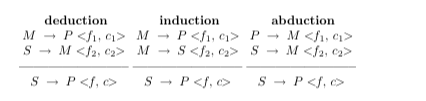
\includegraphics[width=12cm]{figures/nars.png}
\caption{ NARS/PLN term logic deduction, induction and abduction inference forms }
\label{fig:nars}
\end{figure}

\subsection{Cyc系统}{Cyc}

在NLP系统中,也许开发最彻底的“谓语逻辑”是由Cycorp公司开发的商用系统Cyc\cite{Lenat1990}。Cyc系统拥有一个非常丰富的人工编码知识库,它的终极目标是:以谓语逻辑的形式,将所有人类常识进行编码。虽然它的知识库中已存有数百万的谓语逻辑公式,但到目前为止,似乎只对一小部分人类常识进行了编码。 不过,作为智能应用系统,Cyc已经相当成功了。

我们之所以在这里讨论Cyc“知识表示”的基础,是为了与我们的系统进行比较。在Cyc系统中,概念名称被称作“常量”。在书写时,它们以"\#\$"开始。以下是几种常量:

\begin{itemize}
\item 单个词汇被称为“个体词”,例如:\#\$BillClinton (比尔·克林顿 或 \#\$France(法国)。
\item 集合词,例如\#\$Tree(树)-ThePlant(植物) (包括所有的树) 或 \#\$EquivalenceRelation (等价关系)(包括所有的等价关系)。
\item 真值函数,可以运用到一个或多个概念中,并反馈“真”或“假”。例如:\#\$siblings is the sibling relationship,如果两个参数是siblings,那就是真的。按照惯例,真值函数以小写字母开头。真值函数可能会被分拆为逻辑连接词(如:\#\$and, \#\$or, \#\$not, \#\$implies)和量词(如:\#\$forAll, \#\$thereExists等)。
\item “函数”能够从给定的词中生成新词汇,例如:
\#\$FruitFn,当提供了一个描述某种植物类型(或集合)的参数,它会给出这类植物的一组水果。按照惯例,“函数常量”以“大写字母”开始,以字符“Fn”结束。
\end{itemize}

“常量”之间由谓语联系在一起。最重要的谓语是: \#\$isa 和 \#\$genls。第一个(\#\$isa)描述的是:某个个体是某个集合中的一个例子(如:specialization);第二个(\#\$genls)描述的是:一个集合是另一个集合的子集合(例如:generalization)。
利用特定的CycL句子,我们可以得出概念事实。谓语是写在它的参数之前的,在圆括号内。例如:

 {\tt\begin{small}\begin{lstlisting}
    (\#\$isa \#\$BillClinton \#\$UnitedStatesPresident) \;
    \end{lstlisting}\end{small}}

\noindent 意思是 "Bill Clinton belongs to the collection of U.S. presidents" ;

 {\tt\begin{small}\begin{lstlisting}
    (\#\$genls \#\$Tree-ThePlant \#\$Plant) \;
    \end{lstlisting}\end{small}}
    
\noindent 意思是 "All trees are plants"; and 

 {\tt\begin{small}\begin{lstlisting}
    (\#\$capitalCity \#\$France \#\$Paris) \;
    \end{lstlisting}\end{small}}
    
\noindent 意思是 "Paris is the capital of France."


下面是比较封复杂的例子,它表示了一组或一类词的规则,而不是任意特定的个别词:

 {\tt\begin{small}\begin{lstlisting}
 (\#\$relationAllExists \#\$biologicalMother 
 \#\$ChordataPhylum \#\$FemaleAnimal)
    \end{lstlisting}\end{small}}
    

Cyc知识库被分为多个“微理论”库,它们是概念和事实的集合,每个“微理论”库都与一个特定领域相关联。每个“微理论”库都不能有相互矛盾的信息,而且可以通过Bayesian网络提供概率真值。

Cyc配备了一个复杂的、基于短语结构语法的NLP系统,这个系统将自然语言句子映射为Cyc逻辑形式。由于这个系统本身的特性,我们尚不清楚它到底具有什么样的优点和缺点。


\subsubsection{ConceptNet}{ConceptNet}

知识表示的另一个模式是由ConceptNet提供的\cite{Liu2004}。它从Cyc系统和形式逻辑中借鉴了一些理念,但没有考虑复杂的位元,如量词,并且比较接近自然语言层面。ConceptNet 是个大规模的语义网络,它表达概念(由单词或短语表述)之间的关系。图\ref{fig:concept}是关于子网络的例子。

\begin{figure}[htb]
\centering
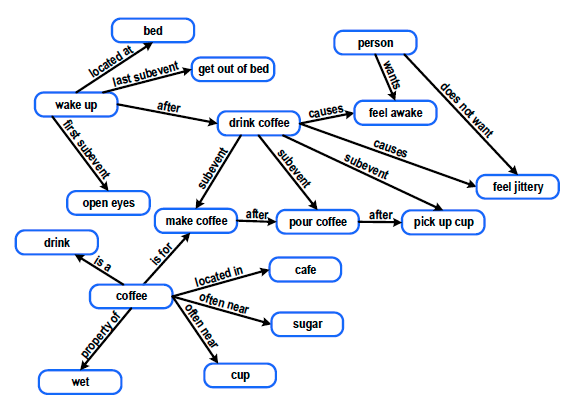
\includegraphics[width=12cm]{figures/conceptnet.png}
\caption{ An illustrative fragment of ConceptNet }
\label{fig:concept}
\end{figure}

ConceptNet系统的节点是自然语言碎片,这些碎片按照某个句法模式的本体进行了半结构化。它们适合一阶概念(作为名词短语,如potato chips)和二阶概念(作为动词短语,如:buy potato chips)。

节点可以由19个语义关系相连接:
\begin{itemize}

\item 事物 
\begin{itemize}
\item IsA ?(corresponds loosely to hypernym in WordNet)
\item PropertyOf ?(e.g. (PropertyOf ``apple'' ``healthy''))
\item PartOf ?(corresponds loosely to holonym in WordNet)
\item MadeOf ?(e.g. (MadeOf ``bottle'' ``plastic''))
\end{itemize}

\item 事件 
\begin{itemize}
\item FirstSubeventOf, LastSubeventOf ?(e.g. (FirstSubeventOf ``act in play'' ``learn script''))
\item EventForGoalEvent ?(e.g. (EventForGoalEvent ``drive to grocery store'' ``buy food''))
\item EventForGoalState ?(e.g. (EventForGoalState ``meditate'' ``enlightenment''))
\item EventRequiresObject ?(e.g. (EventRequiresObject ``apply for job'' ``resume''))
\end{itemize}

\item 动作 
\begin{itemize}
\item EffectOf ?(e.g. (EffectOf ``commit perjury'' ``go to jail''))
\item EffectOfIsState ?(e.g. (EffectOfIsState ``commit perjury'' ``criminal prosecution''))
\item CapableOf ?(e.g. (CapableOf ``police officer'' ``make arrest''))
\end{itemize}

\item 空间 
\begin{itemize}
\item OftenNear ?(e.g. (OftenNear ``sailboat'' ``marina''))
\item LocationOf ?(e.g. (LocationOf ``money'' ``in bank account''))
\end{itemize}

\item 目标 
\begin{itemize}
\item DesiresEvent, DesiresNotEvent ?(e.g. (DesiresEvent ``child'' ``be loved''))
\end{itemize}

\item 功能
\begin{itemize} 
\item UsedFor ?(e.g. (UsedFor ``whistle'' ``attract attention''))
\end{itemize}

\item 通用 
\begin{itemize}
\item CanDo ?(e.g. (CanDo ``ball'' ``bounce''))
\item ConceptuallyRelatedTo ?(e.g. (ConceptuallyRelatedTo ``wedding'' ``bride'' ``groom'' )
\end{itemize}
\end{itemize}


OpenCog的Atomspace是本文的研究重点,它与ConceptNet有些共同之处。我们视Atomspace为“加权标记超级图”,但ConceptNet只是一个“加权标记图”。此外,在可以直接表示的关系复杂性方面,Atomspace与ConceptNet有所不同。Atomspace包含与ConceptNet相似的简单节点和链接,但还有更加复杂的,且能够表示量词关系,还含有可执行程序等。它的设计原则是:先利用简单的、ConceptNet类的方法,尽可能地表示,但之后在必要的情况下使用更复杂的表示工具。大多数“表示工具”都来自传统逻辑,而不是谓语逻辑,但必要时也使用与“明确量词关系”相对应的节点和链接。


\section{语言生成}{Generation}

自然语言生成(NLG)是NL的反向过程。NLG是从信息的计算表示中自动生成人类(自然的)语言。大体上,NLG系统与以下问题有关:

\begin{itemize}
\item What should I say?(我应该说什么?)
\item How should I say it?(我应该怎么说?)
\end{itemize}

这涉及许多相互关联的计划过程,如:
\begin{itemize}
\item 决定要说的信息
\item 构建语篇计划
\item 将信息块转换为语篇单位
\item 选择适当的短语和单词
\item 输出正确的语法
\end{itemize}

将这个流程分解为阶段的方法如下:
\begin{enumerate}
\item 宏观计划
\item 微观计划
\item 表层实现
\end{enumerate}

宏观计划涉及选择和组织内容。它输入的是一个或多个沟通目标:解释、描述,或提问;引起听众的某种行动或思考等。宏观计划输出的是一种知识架构,这个架构不一定是语言的属性,而是体现智能体所要沟通的信息。除了一般性内容,这种知识架构可能包含一些与沟通过程有关的信息,例如:不同的知识块应该以什么样的顺序来传达。

有些宏观计划法涉及语篇结构的特定理论,例如:修辞结构理论\cite{Mann1987}。在本文所介绍的研究中,我们采用了宏观计划,利用名为“OpenPsi”的“动机认知模型”(这个模型的构建密切遵循人类心理学)。

微观计划则运用知识架构,并将它们分为句块。微观计划必须处理多种语言问题,例如:

\begin{itemize}
\item 句子范围:是否可以将两片叶子接在一起,怎样接在一起。(“我今天饿了。我去了 Burger King。” VS “我今天饿了,所以我去了Burger King。”)
\item 代词化
\item 聚合:删除重复内容。(“抽烟对你不好。抽烟会缩短你的寿命。抽烟让你口气不佳” VS “抽烟对你不好、缩短你的寿命,而且让你口气不佳”)
\item 主题化
\item 主题排序
\end{itemize}

到目前为止,我们的大多数微观计划都是为特定的应用而专门制定的。有一个名为SPUD\cite{Stone 1997}的多用途微观计划框架,它利用的是一个基于逻辑的计划流程形式。尽管在细节上有所不同(原来的SPUD是基于树-邻近语法),但我们所描述的微观计划在概念上受到了SPUD的很大影响。

最后,“表面实现”涉及的是文本表层的生成,例如:把知识结构转换为句子。经典的表层生成器,例如FUF/SURGE\cite{Elhadad1992}和 Penman/KPML\cite{Matthiessen1991},都是以深层语言学理论为基础的。其他知名的系统,例如Nitrogen\cite{Langkilde1998}则采用的是统计法。所有基于规则的方法和统计法现在仍然流行。

一般来说,与NL理解相比,NL生成技术要落后得多。目前的实用系统往往比较专业化,而且很粗糙。概念比较先进的系统,如FCG,尚未经过广泛地实践测试。正如第\ref{chap:generation}章中所介绍的,我们在这一领域的研究代表了“基于规则的方法”和“统计法”的融合。我们认为这种融合非常有前景,但还没有精细化,也没有经过系统性评估。

\section{问题回答}{Question Answering}

就连接NL理解、生成和知识表示而言,也许最简单、最有意义的模式就是“问题回答”。问答(QA)系统让使用者以自然语言提问,然后以自然语言响应。


许多现代QA系统基本上都是以文档为驱动的信息检索系统,请见图\ref{fig:qa}中的示例\cite{Hirschman2001}。这种系统(其中的问题被直接提交至一个大规模文本语料库)的表现通常优于20世纪70年代的早期QA系统(依赖人工编码的知识库)。

\begin{figure}[htb]
\centering
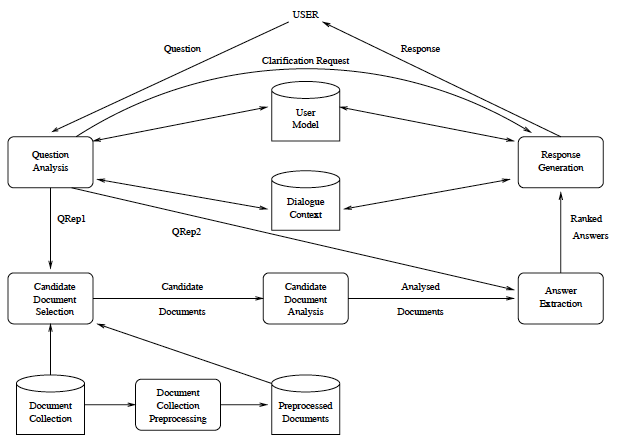
\includegraphics[width=12cm]{figures/qa.png}
\caption{典型的文件驱动问答系统的架构}
\label{fig:qa}
\end{figure}

这种以文件为驱动的QA系统通常包括一个问题分类模块。这个模块确定问题和回答的类型。分析问题之后,系统一般会运用几个模块。文本的数量逐步减少,这些模块则越来越多地应用于复杂的NLP技术。因此,文件检索模块可以使用搜索引擎来识别那些可能含有“答案”的文件,或文档中的段落。随后,一个过滤器预先挑选出包含同类字符的小文本碎片,用作预期回答。例如:如果问题是“谁发明了青霉素?”,过滤器会反馈包含人名的文本。最后,一个“回答抽取模块”会在文本中进一步寻找线索,以确定候选的答案是否能正确地回答这个问题。

另一方面,如果问答系统会根据对文本知识的深层理解来做出响应,那么“快速处理文本来响应问题”就不是一个非常可行的策略。更准确地说,用于为QA系统提供知识的文件必须预先由一个NL理解系统彻底地“读”和理解。后面的那个方法是我们要在本文的第\ref{chap:dialogue}章中探讨的。我们开发了一个简单的QA系统,它是一个整体互动对话体系的一部分。

在2010年,IBM的问答系统Watson以极大的优势击败了另两个Jeopardy冠军奖的获得者:Brad Rutter 和 Ken Jennings。Watson综合利用了信息检索法和基于推理的先进方法\cite{Ferrucci2011},可以说是迄今为止最先进的问答系统。

\subsubsection{问答系统的关键问题}{Key Issues Regarding Question Answering}

问答系统是一个复杂的探索课题,它涉及众多问题。举例来说,有证据表明:某种问题要难于其它问题。询问“为什么”和“怎样”的问题往往比询问“是什么”和“在哪里”的问题更难回答,这是因为它们要求对因果关系,或instrumental关系的理解。这些关系通常由分句或独立的句子来表达\cite{Hirschman1999}。

在2002年,一组研究人员绘制了一幅关于问答系统的研究路线图\cite{Burger2002}。他们当时提出的问题在今天仍然与我们息息相关。以下是他们发现的问题:

\begin{itemize}
\item 问题类别:不同类型的问题(例如“列支敦士登的首都是哪里?” VS“为什么会形成彩虹?”VS“玛丽莲·梦露和加里·格兰特出演过同一部电影吗?”)要求使用不同的策略来发现答案。
\item 问题处理:相同的信息可能是用不同的方式 来表达的,有些是疑问句(“莱索托国的国王是谁?”),有些是祈使句(“告诉我莱索托国王的名字。”)。因此,梳理出有效信息需要花些功夫。
\item 上下文和问答:上下文可能用于厘清某个问题、解决歧义,或者追踪一系列问题的调查。(例如“为什么Joe Biden2010年访问了伊拉克?”。这个问题也可能这样问:为什么副总统Biden去访问,而不是Obama总统;为什么他去的是伊拉克,而不是阿富汗或其他国家;为什么他是2010年去的,而不是在那之前或之后;或者Biden希望在那次访问中取得什么成果等。)
\item 回答公式:QA系统生成的结果以尽可能自然的方式呈现。
\item 实时问答:不论问题有多复杂,“快速回答”在实际应用中都非常重要。
\item 互动问答:经常出现的一种情况是:QA系统没有很好地获取信息需求,因为问题处理部分可能没有成功地对需要抽取的问题或信息进行正确分类,而且生成答案也不容易检索。在这种情况下,提问的人可能不仅想重新表达问题,还想与系统进行对话。此外,系统也可以利用之前回答过的问题。
\item 先进的QA推理:更多复杂的问题等待着书面文本或结构数据库以外的回答。为了完善QA系统,在其中添加这些功能,以下几项工作是必要的:整合推理模块、建立多种知识库、对通用知识,常识推理机制,以及不同领域的特定知识进行编码。我们的研究正是要推动这方面的发展。
\item QA用户归档:用户归纳是用于获取提问者的数据,包括上下文数据、兴趣、提问者常用的推理方案、系统和使用者之间不同对话的共同点等。这种归档可以为QA系统的表现提供有价值的指引。
\end{itemize}

另一个与QA有关的问题是:如何判断某个“回答”的质量。以下是几个常用标准:

\begin{itemize}
\item 相关性:“回答”应该是对问题的响应。
\item 正确性:“回答”应该符合事实。
\item 简洁性:“回答”不应该包括无关信息。
\item 完整性:“回答”应该完整,例如:不完整的回答不应该得满分。
\item 连贯性:“回答”应该是连贯的,这样才能方便提问者阅读。
\item 正当理由:“回答”中应该带有足够的上下文,以便提问者了解为什么选择了这个答案。
\end{itemize}

到目前为止,大多数研究都关注了“相关性”。

\section{对话系统}{Dialogue Systems}

Tursing(图灵)曾在其1950年的论文中阐述了他对终极NLP应用的预期:对话系统能够以自然的方式与人类使用者进行谈话。粗糙的对话系统(如:Apple的SIRI),在今天已成为我们日常生活的一部分,但真正具有人类思维能力的对话系统仍然没有实现其研究目标。

图\ref{fig:dialogue}描述了对话系统的通用结构\cite{Arora2013}。除了NL生成和理解,以及从各种资源中获取相关知识,其主要模块是对话管理器。这个模块决定在谈话中的每个节点说什么。

\begin{figure}[htb]
\centering
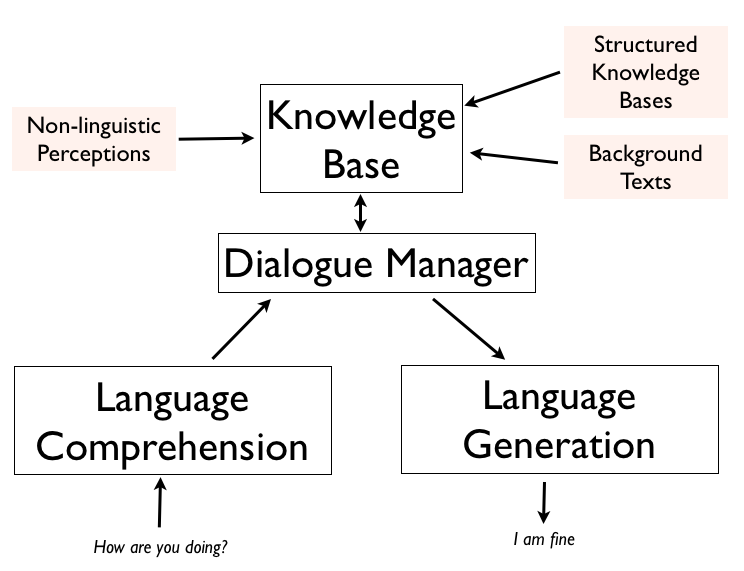
\includegraphics[width=12cm]{figures/dialogue_system.png}
\caption{ A generic dialogue-system architecture }
\label{fig:dialogue}
\end{figure}

总之,对话管理器全方位管理对话。它采用用户文本的语义表示、确定文本是否契合上下文,并构建系统响应的语义表示。一般来说,在它的职责中,以下几个是必要的:

\begin{itemize}
\item 保存对话历史
\item 采用一定的对话策略
\item 处理格式错误和无法识别的文本
\item 检索文件或数据库中的内容
\item 确保为使用者提供最好的响应
\item 管理启动和系统响应
\item 处理语言学问题
\item 言语分析
\item 以任何可用的、相关的非语言信息来构建语言结构。
\end{itemize}

目前大多数对话系统都利用一小部分固定规则来处理对话管理(这些规则代表人工制定的言语策略)。近年的一些系统还提供另一种方法:利用概率模型(如:POMDP)来控制对话,但这些系统还不具备有价值的实用性\cite{Young2006} \cite{Williams2010}。

\begin{figure}[htb]
\centering
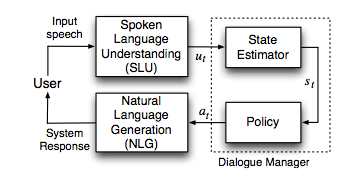
\includegraphics[width=12cm]{figures/pomdp.png}
\caption{ A POMDP-based reinforcement-learning-driven dialogue-system architecture }
\label{fig:dialogue}
\end{figure}


%%%%%%%%%%%%%%%%%%%%%%%%%%%%%%%%%%%%%%%%%%%%%%%%%%%%%%%%%%%%%%%
\subsection{言语行为论}{Speech Act Theory}
\label{sec:speechAct}
%%%%%%%%%%%%%%%%%%%%%%%%%%%%%%%%%%%%%%%%%%%%%%%%%%%%%%%%%%%%%%%

分析“对话系统”需要生成的各类话语的一个方法是:使用由Austin\cite{Austin2005}和Searle\cite{Searle1969} 开创,又经他人进一步完善的“言语行为论”。本文所阐述的对话研究中使用的正是这种方法。我们在这里先回顾非常基本的言语行为论,然后介绍言语行为论的具体变化。在研究过程中,我们发现这个理论是极有用的。

言语行为论的核心概念是:分析不连续言语行为的语言学行为,以实现特定的目标。在OpenCog环境下,这是一种使用方便的理论方法,因为它促使我们像对待OPenCog系统实施的其它行为一样对待言语行为,并推动我们通过标准的OpenCog行为选择机制来处理言语行为。

\begin{itemize}
\item {\bf 言语行为论}:探讨那些可以通过言语来表现的行为类型。
\item {\bf 言表意的行为}:某句话的外在表现,例如:真实言语和它的表面含义。
\item {\bf 言外行为}:言语的“言外之力”,例如它的目标含义(作为社交层面的有效言语行为)。(按照Searle的使用方法,“言语行为”有时仅仅指的是言外行为。我们不用这个方法。)
\item {\bf 言后行为}:它的实际效果,例如:说服、劝说、吓唬、启发、激励,或者让某人做或实现某个事项,不论是有意或无意的。
\end{itemize}

在Searle看来,说话人通过他们的言语,只能获得5类言外之力,分别是:

\begin{itemize}
\item 断言类:说话人自己承诺事情是真的。The sky is blue (天是蓝色的)
\item 指令类:说话人试图让受话人做某事。Clean your room! (打扫你的房间!)
\item 承诺类:说话人对未来的行为做出承诺。I will do it (我将会做这件事)
\item 表达类:说话者表达了某些心理状态。I’m Sorry (对不起)。
\item 声明类:说话人带来了不同的状况。The meeting is adjourned.(这个会议休会了)。
\end{itemize} 

受这个本体论的启发,Twitchell 和 Nunamake在他们2004年的论文(标题为:言语行为归档:分析持续谈话和其参与者的概率统计法。\cite{Twitchell2004})中提出了更加精细的“42种言语行为”本体论,叫做SWBD-DAMSL (DAMSL = Dialogue Act Markup in Several Layers)。尽管有少量不符合Searle的观点,并被分类为“其它”,但几乎他们所有的42种言语行为类型都能够被映射到Searle的5个高级类别之一。图\ref{fig:DAMSL}和\ref{fig:Searle}描述了这42种行为和它们与Searle分类之间的关系。我们已经利用了这个Searle解析法,它给我们正在进行的自然语言对话研究带来了灵感。

\begin{figure}[htb]
\centering
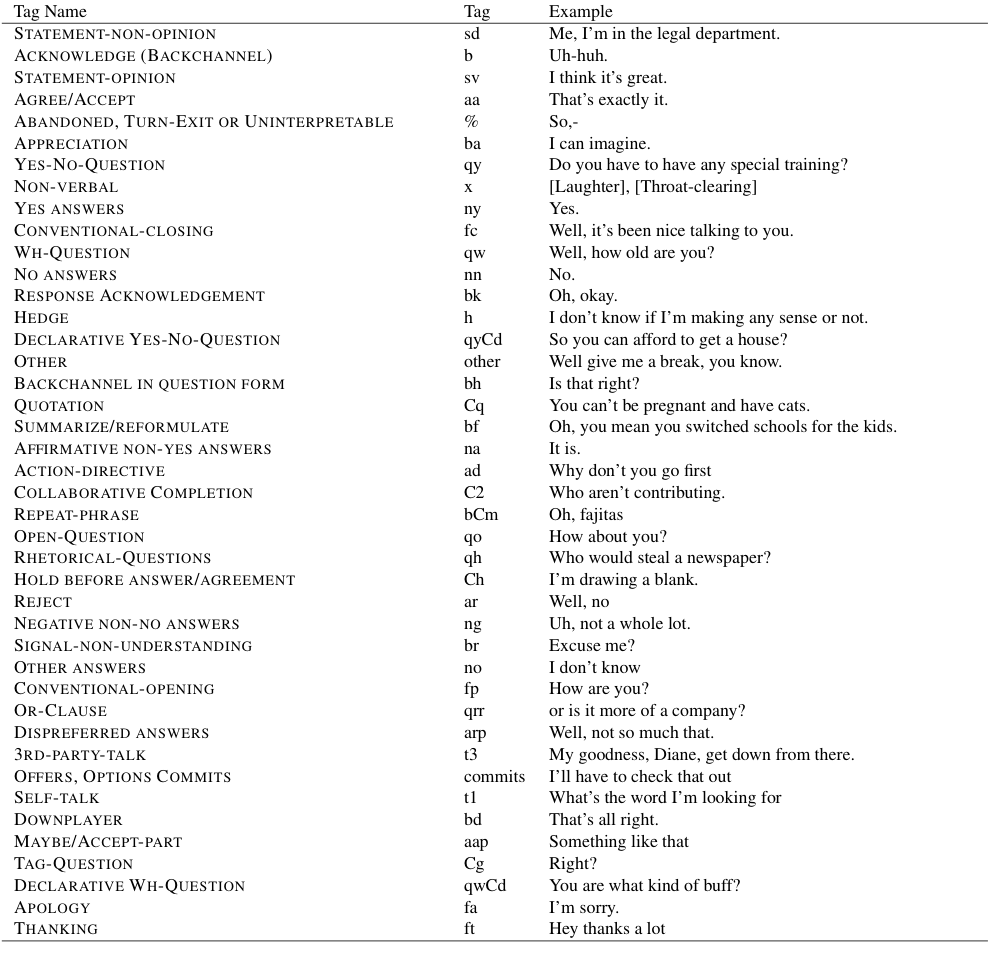
\includegraphics[width=12cm]{figures/DAMSL.png}
\caption{ The 42 speech acts presented in the SWBD-DAMSL study}
\label{fig:DAMSL}
\end{figure}

\begin{figure}[htb]
\centering
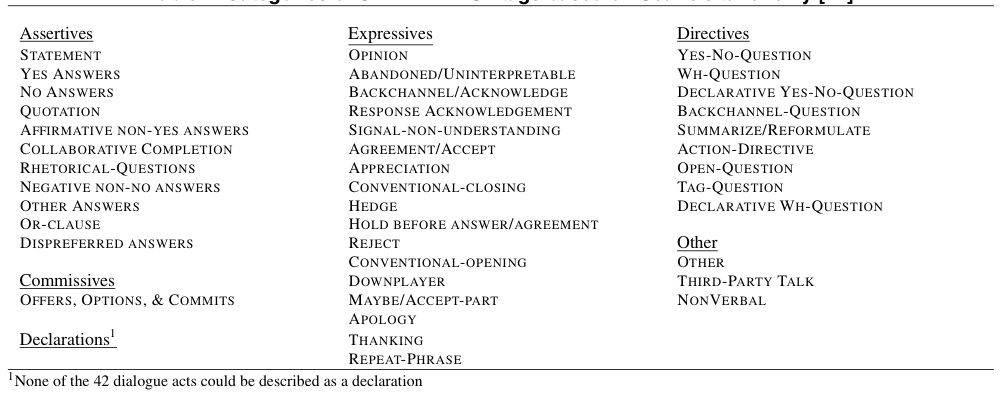
\includegraphics[width=12cm]{figures/Searle.png}
\caption{ Correlation of the 42 SWBD-DAMSL speech acts with Searle's high-level speech act categories }
\label{fig:Searle}
\end{figure}

1.6.2 CogDial架构

在第??章的图??中,我们粗略地介绍了我们自己的对话架构。按照我们的方法,对话管理是通过一个通用动机认知模型来实施的,我们称之为“OpenPsi”。“知识”从我们的NL理解系统中分配到OpenCog的Atomspace知识存储中,然后OpenPsi会根据某一特定时间点的系统目标,从大量“言语行为模式”中选择一个,并用它来指导其余的宏观计划过程。随后,被选中的“言语行为模式”利用PLN推理和其它工具,实施认知处理,并收集知识组(例如:Atomspace中的原子、节点和链接),再将其分配到NL生成子系统中,以转换为英语。这个复杂的架构代表了人工编码和学习模块的融合。
 
(24和25页都是不需要翻译的图表)
